\documentclass[a4paper]{article}
\usepackage[T1]{fontenc}
\usepackage[utf8]{inputenc}
% \usepackage[swedish]{babel}
\usepackage{fancyvrb}
\usepackage{graphicx}
\usepackage{biblatex}
\usepackage{verbatim}
\usepackage{listings}
\usepackage{xcolor}
\usepackage{url}
\usepackage{amsmath}

\addbibresource[]{assignment3.bib}
\fvset{tabsize=4}
\fvset{fontsize=\small}

\definecolor{codegreen}{rgb}{0,0.6,0}
\definecolor{codegray}{rgb}{0.5,0.5,0.5}
\definecolor{codepurple}{rgb}{0.58,0,0.82}
\definecolor{backcolour}{rgb}{0.95,0.95,0.92}
\lstdefinestyle{mystyle}{
    backgroundcolor=\color{backcolour},   
    commentstyle=\color{codegreen},
    keywordstyle=\color{magenta},
    numberstyle=\tiny\color{codegray},
    stringstyle=\color{codepurple},
    basicstyle=\footnotesize,
    breakatwhitespace=false,         
    breaklines=true,                 
    captionpos=b,                    
    keepspaces=true,                 
    numbers=none,                    
    numbersep=5pt,                  
    showspaces=false,                
    showstringspaces=false,
    showtabs=false,                  
    tabsize=2
}
\lstset{style=mystyle}

\title{TFRP20 Artificial Intelligence (VT25)\\ Assignment 3: Classification with the perceptron and logistic regression}
\author{Anders Holm\\\texttt{anders.holm@senspix.net} \and
Magnus Gäfvert\\\texttt{magnus.gafvert@gmail.com}}
\date{2025--03--10}
\begin{document}
\maketitle
\begin{abstract}
    This report present and discuss the authors' solution to the assignment on classification with the perceptron and logistic regression. The solution is implemented in the given template Jupyter notebook and provided alongside this report.
\end{abstract}

\section{Introduction}
The objectives of this assignment~\cite{tfrp20assignment3} are to:

\begin{enumerate}
    \item  Write a linear regression program using gradient descent;
    \item  Write linear classifiers using the perceptron algorithm and logistic regression;
    \item  Experiment variations of the algorithms;
    \item  Evaluate classifiers;
    \item  Experiment with popular tools;
    \item  Read a scientific article on optimization techniques and comment it;
    \item  Present code, results, and comments in a short dissertation. 
\end{enumerate}

The respective tasks are presented in the following sections.

\section{Method}
The implementation toolchain is based on Jupyter Notebook with Python 3.9.21 and the Anaconda distribution~\cite{anaconda} using Microsoft Visual Studio Code with free GitHub Copilot served by the preview Anthropic Claude 3.5 Sonnet LLM and Microsoft Python plugins. This report is typeset with \LaTeX using TexLive and and the LaTeX Workshop plugin by James Yu.

The code is structured in a Jupyter notebook 
\begin{verbatim}
    ai_lab_perceptron_students.ipynb    
\end{verbatim}
with sections and cells for each of the tasks in the assignment. The code is evaluated with the provided evaluation data from the historial novel Salammbô by Gustave Flaubert~\cite{flaubert1862salammbô} to verify performance of the implementation.

 
\section{Results and discussion}


\subsection{Linear regression program using gradient descent}

\begin{figure}
    \centering
    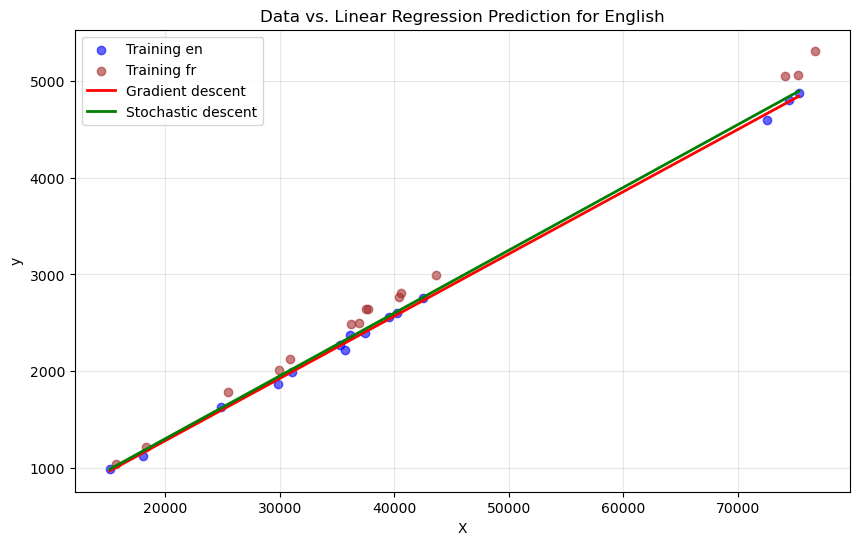
\includegraphics[width=0.8\textwidth]{figures/Fit English.png}
    \caption{Screenshot of the Jupyter notebook with the implementation of the perceptron algorithm.}
    \label{fig:regression_English}
\end{figure}

\begin{figure}
    \centering
    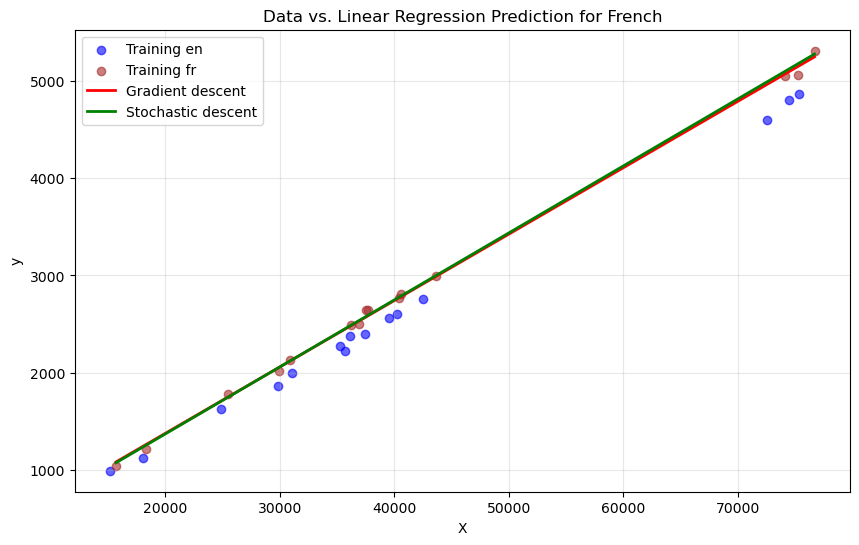
\includegraphics[width=0.8\textwidth]{figures/Fit French.png}
    \caption{Screenshot of the Jupyter notebook with the implementation of the perceptron algorithm.}
    \label{fig:regression_French}
\end{figure}

\begin{figure}
    \centering
    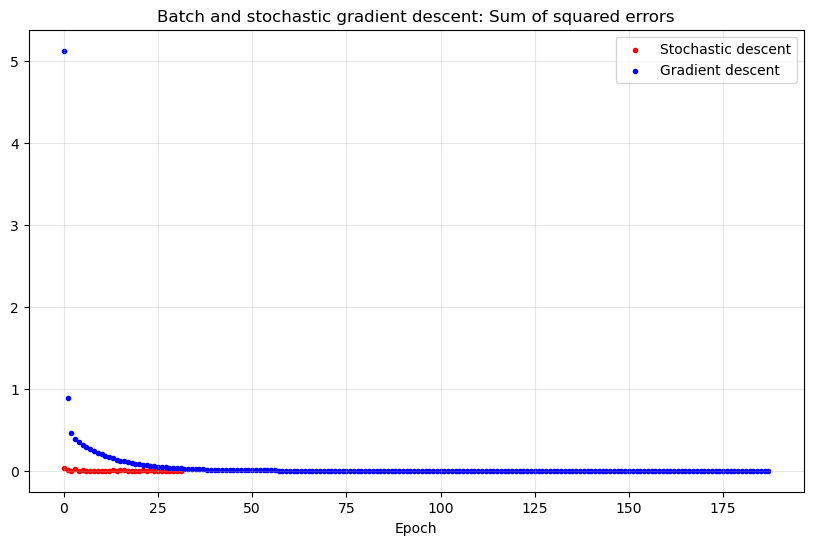
\includegraphics[width=0.8\textwidth]{figures/Regression errors.png}
    \caption{Screenshot of the Jupyter notebook with the implementation of the perceptron algorithm.}
    \label{fig:regression_French}
\end{figure}

\begin{table}[]
    \caption{Regression results}
    \label{tab:regression-table}
    \small
    \begin{tabular}{lllll}
        \hline\hline
             & \multicolumn{2}{c}{French}                    & \multicolumn{2}{c}{English}            \\
             & Gradient descent & Stochastic descent & Gradient descent & Stochastic descent \\
             \hline
    Epoch    & 187              & 31                 & 186              & 15                 \\
    w{[}0{]} & 0.00170945       & -0.00170833        & -6.71530774e-04  & 0.00111656         \\
    w{[}1{]} & 0.98640986       & 0.99526806         & 9.94590530e-01   & 1.00362464\\
    \hline\hline
    \end{tabular}
\end{table}


\subsection{Linear classifiers using the perceptron algorithm and logistic regression}

\begin{figure}
    \centering
    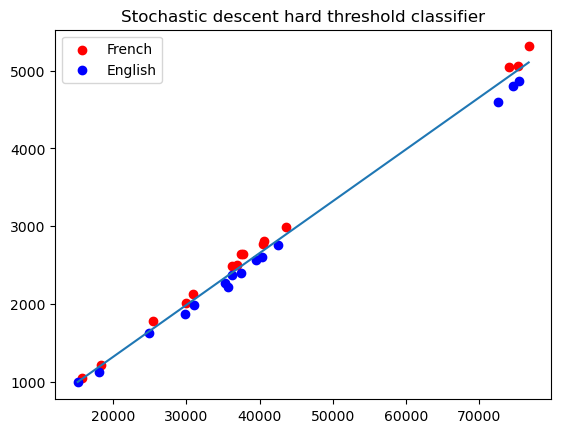
\includegraphics[width=0.8\textwidth]{figures/Stochastic descent hard threshold classifier.png}
    \caption{Screenshot of the Jupyter notebook with the implementation of the perceptron algorithm.}
    \label{fig:Stochastic_descent_hard_threshold_classifier}
\end{figure}

\begin{figure}
    \centering
    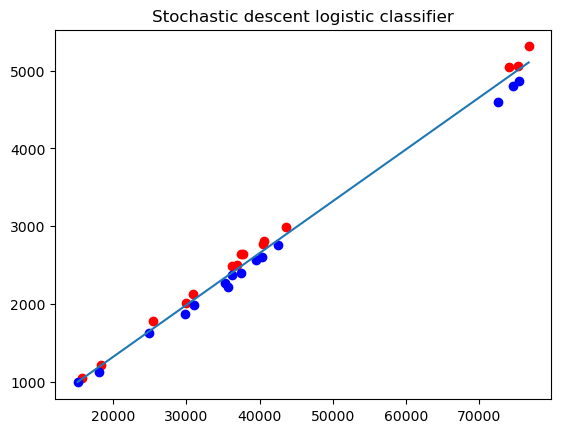
\includegraphics[width=0.8\textwidth]{figures/Stoschastic descent logistic classifier.png}
    \caption{Screenshot of the Jupyter notebook with the implementation of the perceptron algorithm.}
    \label{fig:classifier_result_1}
\end{figure}

\begin{figure}
    \centering
    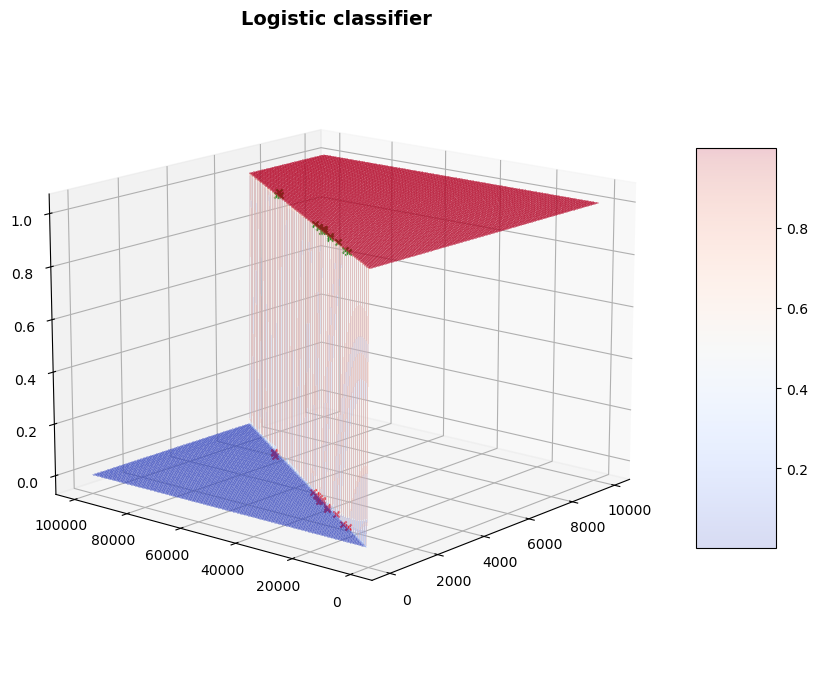
\includegraphics[width=0.8\textwidth]{figures/logistic classifier.png}
    \caption{Screenshot of the Jupyter notebook with the implementation of the perceptron algorithm.}
    \label{fig:classifier_result_2}
\end{figure}


\begin{figure}
    \centering
    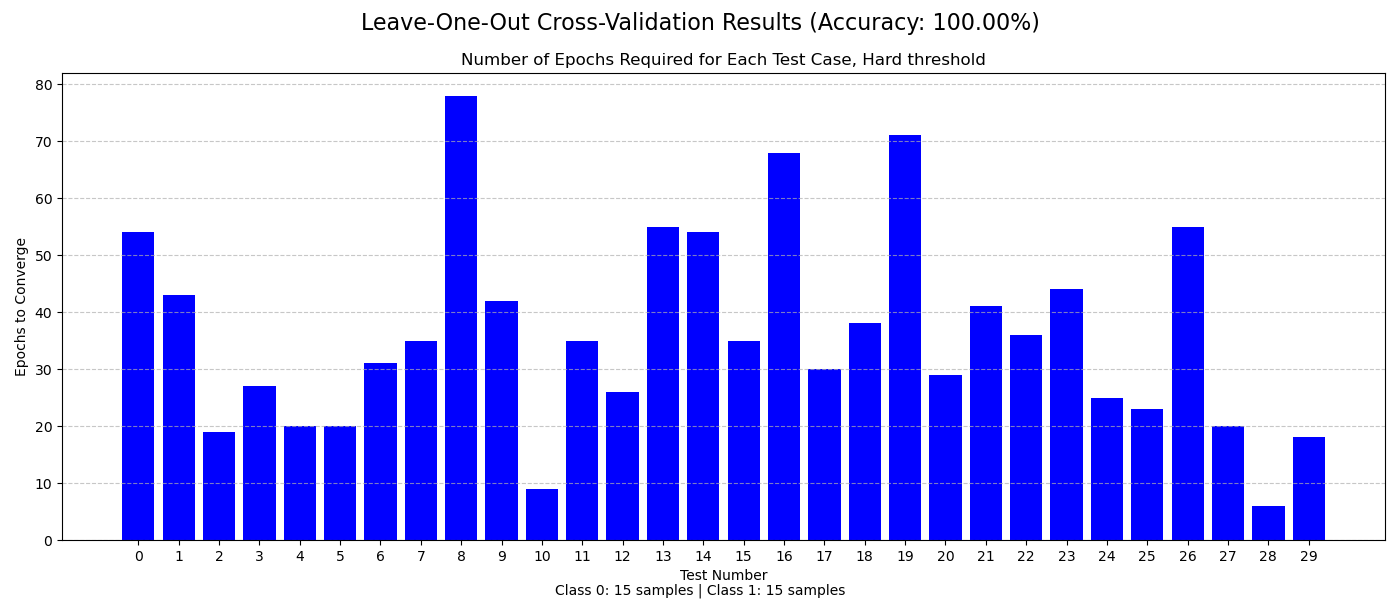
\includegraphics[width=0.8\textwidth]{figures/classifier result 1.png}
    \caption{Screenshot of the Jupyter notebook with the implementation of the perceptron algorithm.}
    \label{fig:classifier_result_1}
\end{figure}

\begin{figure}
    \centering
    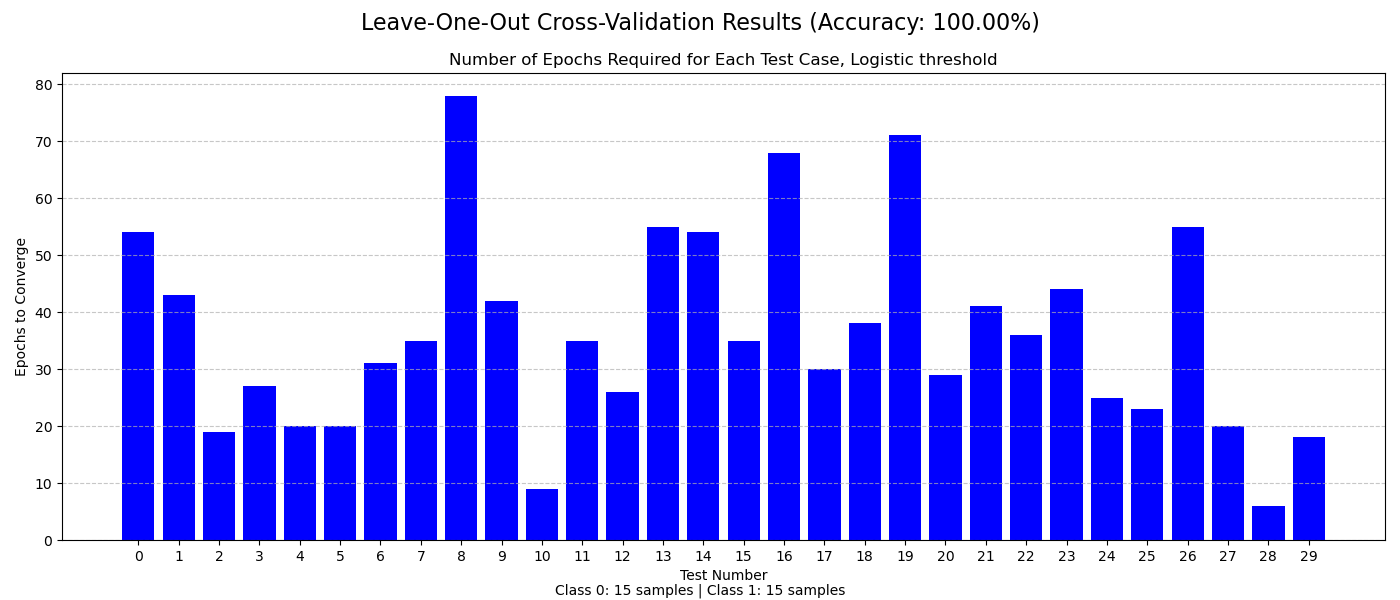
\includegraphics[width=0.8\textwidth]{figures/classifier result 2.png}
    \caption{Screenshot of the Jupyter notebook with the implementation of the perceptron algorithm.}
    \label{fig:classifier_result_2}
\end{figure}


\subsection{Experimenting with popular tools: \texttt{Keras}, \texttt{PyTorch}, \texttt{scikit\_learn}}

\subsection{Reading Ruder}
You will read the article An overview of gradient descent optimization algorithms by Ruder (2017) and you will outline the main characteristics of all the optimization algorithms the author describes. This part should be of about one to two pages. 
\cite{DBLP:journals/corr/Ruder16}


\section{Conclusions and future work}


\printbibliography
\end{document}